\section{Overview}

\subsection{Was ist ein Verteiltes System?}
\begin{itemize}
      \item Vile Dinge könnten unter diese Definition fallen, wie z.B. Mulicore Rechner, Cload Rechner oder ein Heimnetzwerk
      \item In der Lehrveranstaltung wird folgende Definition verwendet:\\
            \quotes{Ein verteiltes System ist eine Ansammlung \textit{unabhängiger Computer}, die den Benutzern wie ein \textit{einzelnes kohärentes} System erscheinen.}
      \item Wie betrachten also keine einzelnen großen Parallelrechner und die Verteilung muss dem Nutzer gegenüber verborgen sein (Transparenz)
\end{itemize}

\subsection{Ziele von verteilten Systemen}
\begin{enumerate}
      \item \textbf{Verteilungstransparenz}:\\
            Die Verteiltheit ist dem Nutzer gegenüber verborgen. Der Nutzer weiß nicht, ob und wie das System verteilt ist. Speziell wird folgendes verborgen:
            \begin{enumerate}
                  \item Zugriff:\\
                        Der Zugriff auf alle Ressourcen erfolgt auf gleichem Weg.
                  \item Ort:\\
                        Man kennt den Ort einer Resource nicht.
                  \item Relokation:\\
                        Resourcen können unbemerkt \textit{während der Nutzung} verschoben werden (z.B. wenn sich der Kommunikationspartner einer Mobilfunkverbindung bewegt)
                  \item Migration:\\
                        Resourcen können unbemerkt \textit{zwischen zwei Zugriffen} den Standort wechseln (Bei Abruf 1 antwortet Server x, bei Abruf 2 antwortet Server y)
                  \item Nebenläufigkeit:\\
                        Trotz eines Mehrnutzerbetriebs einsteht der Eindruck eines Einzelnutzerbetriebs.
                  \item Fehler:\\
                        Der Ausfall einer Komponente wird durch das Ersetzen durch eine andere Komponente verborgen.
            \end{enumerate}
      \item \textbf{Offenheit:}\\
            Das System darf aus heterogenen Komponenten mit unterschiedlichen Technologien (z.B Unterschiedlichen OS, HW, Netzwerkprotokollen) bestehen.
      \item \textbf{Skalierbarkeit:}\\
            Das System soll einfach in seiner Größe erweiterbar sein, um die Power der vorhandenen Komponenten bei steigenden Anforderungen mit neuen Komponenten zu verstärken. Z.B. soll es mehrere Datenbankserver oder Webserver geben können.
            Hierbei soll Portierbarkeit und Erweiterbarkeit gewährleistet werden. Anforderungen könnten sein:
            \begin{itemize}
                  \item zusätzliche Rechenpower
                  \item zusätzliche Nutzer
                  \item zusätzlicher Speicherplatz
            \end{itemize}
      \item \textbf{Zuverlässigkeit:}\\
            Das System soll immer zur Verfügung stehen und möglichst Ausfallsicher sein.
\end{enumerate}

\subsection{CAP Theorem (Brewers Theorem)}
\label{sec:CAP_Theorem}
Dieses Theorem betrachtet die 3 Qualitätseigenschaften/Ziele von verteilten Systemen:
\begin{enumerate}
      \item Konsistenz der Daten
      \item Partitionstoleranz:\\
            ein durch einen Netzwerkfehler in Teilsysteme gespaltenes System kann trotzdem weiter arbeiten
      \item Verfügbarket
\end{enumerate}
Das Theorem sagt aus, dass man nur 2 von diesen 3 Zielen erreichen kann, da sie miteinander in Konflikt stehen.
\\
\\
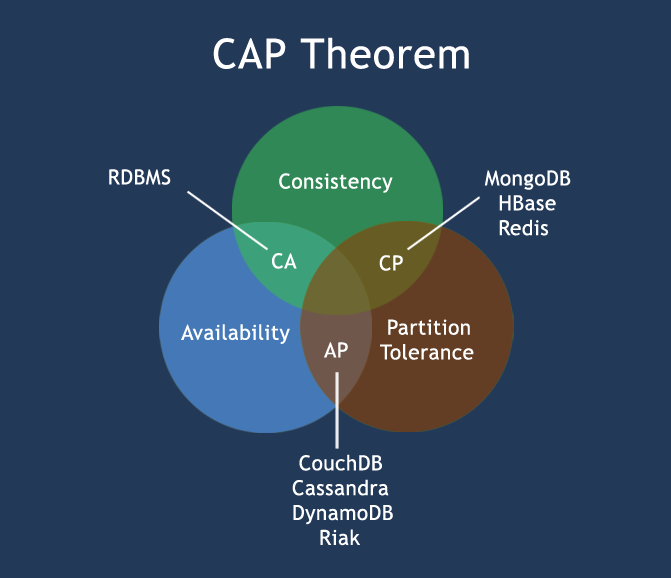
\includegraphics[width=9cm]{CAPTheorem.png}

\subsection{Architekturen für VS}
Ein verteiltes System kann mehreren der folgenden Architekturformen entsprechen. Ein System kann auch heterogen sein und in verschiedenen Teilen verschiedene Architekturen umsetzen.

\subsubsection{Geschichtet (Client-Server)}
Bei einem geschichteten verteilten System werden verschiedene Zuständigkeiten auf mehrere Rechner verteilt. Man unterscheidet zwischen 1-1 Architekturen und Multitier bzw. Multiserver Architekturen.\\
Bei einer \textbf{1-1 Beziehung} wird die Anwendung in genau 2 Teile aufgeteilt. Es handlet sich also, um die klassische Client-Server Architektur. die Anwendung kann hier an beliebigen Teilen unterteilt sein. z.B. kann auf dem Server nur die DB sein, oder auch ein Teil der Anwendung, oder auch noch ein Teil der Benutzerschnittstelle.\\
Eine \textbf{Multitier} Architektur umfasst mehrere Server, die mit einem Client interagieren. Die verschiedenen Schichten, die bei der Informationenverarbeitung durchlaufen werden nennt man auch \textit{layers} oder \textit{tiers}. Es kann z.B. ein \textit{Presentation Layer} geben, dass Daten für den Client darstellt (also wahrscheinlich auf dem Client implementiert z.B. java-script), ein \textit{Service Layer}, das eine API für das Presentation Layer bereitstellt, und ein \textit{Data Access Layer}, das sich um die Daten kümmert (also ein DB Server).

\subsubsection{Objektbasiert}
Objektbasierte Architekturen unterteilen das System in Objekte mit klar definierten Schnittstellen. Ein Objekt kann dann durch Methodenaufrufe auf ein anderes zugreifen. Die Objekte werden dann auf verschiedene Rechner verteilt.\\
Im Gegensatz zur geschichteten Architektur müssen hier also die Schnittstellen noch klarer definiert sein. Die Definitionen überlappen sich aber auch etwas.

\subsubsection{Ereignisbasiert}
Ereignisbasiete Architekturen haben einen Ereignisbus, d.h. ein Kommunikationsmedium, über das Daten asynchron übertragen werden. Wenn ein bestimmtes Ereignis eintrifft, also bestimmte Daten ankommen, kann eine Komponente aktiv werden und die Daten verarbeiten.

\subsubsection{Datenzentriert}
Datenzentrierte Architekturen haben einen gemeinsamen Datenraum (z.B. eine gemeinsame DB), in der Sie sowohl ihre Anfragen als auch Antworten ablegen und so kommunizieren können.